\documentclass[letterpaper]{article}\usepackage[]{graphicx}\usepackage[]{color}
%% maxwidth is the original width if it is less than linewidth
%% otherwise use linewidth (to make sure the graphics do not exceed the margin)
\makeatletter
\def\maxwidth{ %
  \ifdim\Gin@nat@width>\linewidth
    \linewidth
  \else
    \Gin@nat@width
  \fi
}
\makeatother

\definecolor{fgcolor}{rgb}{0.345, 0.345, 0.345}
\newcommand{\hlnum}[1]{\textcolor[rgb]{0.686,0.059,0.569}{#1}}%
\newcommand{\hlstr}[1]{\textcolor[rgb]{0.192,0.494,0.8}{#1}}%
\newcommand{\hlcom}[1]{\textcolor[rgb]{0.678,0.584,0.686}{\textit{#1}}}%
\newcommand{\hlopt}[1]{\textcolor[rgb]{0,0,0}{#1}}%
\newcommand{\hlstd}[1]{\textcolor[rgb]{0.345,0.345,0.345}{#1}}%
\newcommand{\hlkwa}[1]{\textcolor[rgb]{0.161,0.373,0.58}{\textbf{#1}}}%
\newcommand{\hlkwb}[1]{\textcolor[rgb]{0.69,0.353,0.396}{#1}}%
\newcommand{\hlkwc}[1]{\textcolor[rgb]{0.333,0.667,0.333}{#1}}%
\newcommand{\hlkwd}[1]{\textcolor[rgb]{0.737,0.353,0.396}{\textbf{#1}}}%

\usepackage{framed}
\makeatletter
\newenvironment{kframe}{%
 \def\at@end@of@kframe{}%
 \ifinner\ifhmode%
  \def\at@end@of@kframe{\end{minipage}}%
  \begin{minipage}{\columnwidth}%
 \fi\fi%
 \def\FrameCommand##1{\hskip\@totalleftmargin \hskip-\fboxsep
 \colorbox{shadecolor}{##1}\hskip-\fboxsep
     % There is no \\@totalrightmargin, so:
     \hskip-\linewidth \hskip-\@totalleftmargin \hskip\columnwidth}%
 \MakeFramed {\advance\hsize-\width
   \@totalleftmargin\z@ \linewidth\hsize
   \@setminipage}}%
 {\par\unskip\endMakeFramed%
 \at@end@of@kframe}
\makeatother

\definecolor{shadecolor}{rgb}{.97, .97, .97}
\definecolor{messagecolor}{rgb}{0, 0, 0}
\definecolor{warningcolor}{rgb}{1, 0, 1}
\definecolor{errorcolor}{rgb}{1, 0, 0}
\newenvironment{knitrout}{}{} % an empty environment to be redefined in TeX

\usepackage{alltt}
\usepackage[utf8]{inputenc}
\usepackage{amsfonts, amsmath, booktabs, ctable, fixltx2e}
\usepackage[round, authoryear, sort]{natbib}
\usepackage[hidelinks, pdftex, backref=none, bookmarks=true]{hyperref}
\hypersetup{
    pdfauthor = {CAS OSSC},
    pdftitle = {An Introduction to Collaborative Editing Using Repositories},
    pdfsubject = {A sample file to both teach and encourage collaborative editing},
    pdfkeywords = {Git, Open Source, Repository, R, knitr, LaTeX},
    }
\IfFileExists{upquote.sty}{\usepackage{upquote}}{}

\begin{document}


\title{An Introduction to Collaborative Editing Using Repositories}
\author{Open Source Software Committee---Casualty Actuarial Society}
\date{Unpublished}

\maketitle
\begin{abstract}
This paper is intended to serve as a living self-referential document which will describe the process of collaborative editing whilst (and at the same time)\footnote{With apologies to, and deep respect for, the late Peter Sellers\citep{TMS219}} being created through collaborative editing.
\end{abstract}
\section{Introduction}\label{Intro}
Hello. Welcome to the collaborative editing project for the CAS OSSC. This document is meant to be used and abused while learning how to use Git to edit collaboratively. As this is pretty much a fly-by-night attempt to jumpstart collaborative editing, there will certainly be a lot of stumbling along the way. At this point, knowledge of `R', \LaTeX2e{}, the \texttt{knitr} package, and Git is assumed. 

\section{Outstanding Issues}\label{Issues}
\subsection{Bibliography}\label{IssueBib}
One of the issues implied to in section~\ref{Intro} is whether or not the project should have a central bibliography. Those of us who have used \LaTeX{} before probably have a bibliography file (BibTeX or otherwise) numbering in the hundreds of entries. Of course, all of the keys are unique to the files' authors. For this document as of now, individual entries will be added longhand instead of a link to a \texttt{.bib} file.

\section{Some Mathy Stuffs}\label{Maths}
What is a \LaTeX{} document without math and `R' code?

The probability density function for the lognormal distribution is:
\begin{equation}
\frac{1}{x\sigma\sqrt{2\pi}}e^{\frac{\left(\ln{x}-\mu\right)^2}{2\sigma^2}}
\end{equation}

Generating some variates, a summary, and some plots below. It is often good practice to separate the code from the results, so the code will be evaluated and echoed in different blocks. The code that will be used is:
\begin{knitrout}
\definecolor{shadecolor}{rgb}{1, 1, 1}\color{fgcolor}\begin{kframe}
\begin{alltt}
\hlkwd{set.seed}\hlstd{(}\hlnum{764237}\hlstd{)}
\hlstd{Data} \hlkwb{<-} \hlkwd{rlnorm}\hlstd{(}\hlnum{10000}\hlstd{,} \hlkwc{meanlog} \hlstd{=} \hlnum{14}\hlstd{,} \hlkwc{sdlog} \hlstd{=} \hlnum{0.2}\hlstd{)}
\end{alltt}
\end{kframe}
\end{knitrout}

\begin{knitrout}
\definecolor{shadecolor}{rgb}{1, 1, 1}\color{fgcolor}\begin{kframe}
\begin{alltt}
\hlkwd{summary}\hlstd{(Data)}
\end{alltt}
\end{kframe}
\end{knitrout}

\begin{knitrout}
\definecolor{shadecolor}{rgb}{1, 1, 1}\color{fgcolor}\begin{kframe}
\begin{alltt}
\hlkwd{library}\hlstd{(MASS)}
\hlkwd{truehist}\hlstd{(Data,} \hlkwc{nbins} \hlstd{=} \hlstr{"fd"}\hlstd{)}
\hlkwd{lines}\hlstd{(}\hlkwd{density}\hlstd{(Data),} \hlkwc{col} \hlstd{=} \hlstr{"red"}\hlstd{,} \hlkwc{lwd} \hlstd{=} \hlnum{2}\hlstd{)}
\end{alltt}
\end{kframe}
\end{knitrout}

Now to run the code.


\begin{knitrout}
\definecolor{shadecolor}{rgb}{1, 1, 1}\color{fgcolor}\begin{kframe}
\begin{verbatim}
##    Min. 1st Qu.  Median    Mean 3rd Qu.    Max. 
##  563000 1050000 1200000 1220000 1370000 2780000
\end{verbatim}
\end{kframe}
\end{knitrout}

\begin{knitrout}
\definecolor{shadecolor}{rgb}{1, 1, 1}\color{fgcolor}
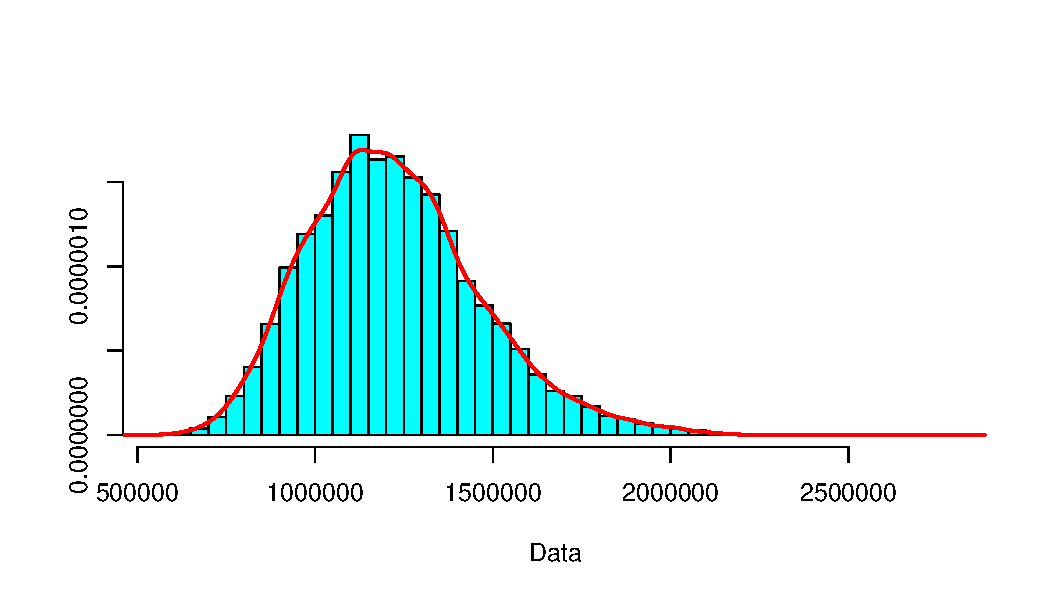
\includegraphics[width=\maxwidth]{figure/Logplot} 

\end{knitrout}

\clearpage
\section{References}\label{Refs}
\bibliographystyle{plainnat}  

\begin{thebibliography}{1}
\providecommand{\natexlab}[1]{#1}
\providecommand{\url}[1]{\texttt{#1}}
\expandafter\ifx\csname urlstyle\endcsname\relax
  \providecommand{\doi}[1]{doi: #1}\else
  \providecommand{\doi}{doi: \begingroup \urlstyle{rm}\Url}\fi

\bibitem[{The Muppet Show}(1977)]{TMS219}
{The Muppet Show}.
\newblock {E}pisode 219.
\newblock Premiered on CBS, 1977.

\end{thebibliography}

\end{document}
